\documentclass[11pt,a4paper]{article}
\usepackage[T1]{fontenc}
\usepackage[english]{babel}
\usepackage{lmodern}
\usepackage[margin=23mm]{geometry}
\usepackage{amsmath,amssymb,booktabs,array,longtable,xcolor,hyperref,fvextra,tikz}
\usetikzlibrary{arrows.meta,positioning}
\hypersetup{colorlinks=true,linkcolor=teal!60!black,urlcolor=blue!60!black,pdftitle={Understanding every function in piret_sm4.py},pdfauthor={Guilherme Martins Specht}}
\fvset{fontsize=\small,breaklines=true,breakanywhere=true}
\newcommand{\hx}[1]{\texttt{#1}}
\newcommand{\hex}[1]{\texttt{#1}}
\newcommand{\xor}{\mathbin{\oplus}}
\newcommand{\rol}{\operatorname{ROL}}
\newcommand{\note}[1]{\par\medskip\noindent\fcolorbox{teal!60!black}{teal!3}{\parbox{\dimexpr\linewidth-2\fboxsep-2\fboxrule\relax}{#1}}\par\medskip}
\setlength{\emergencystretch}{3em}
\setcounter{tocdepth}{1}
\begin{document}
\hypersetup{pageanchor=false}
\begin{titlepage}\centering
\vspace*{20mm}
{\Large Polytech Montpellier --- PFE 5A\par}
\vspace{15mm}
{\Huge\bfseries Understanding Every Function in\par}
\vspace{5mm}
{\LARGE\texttt{piret\_sm4.py}\par}
\vspace{12mm}
{\Large A practical, step-by-step reading guide\par}
\vspace{10mm}
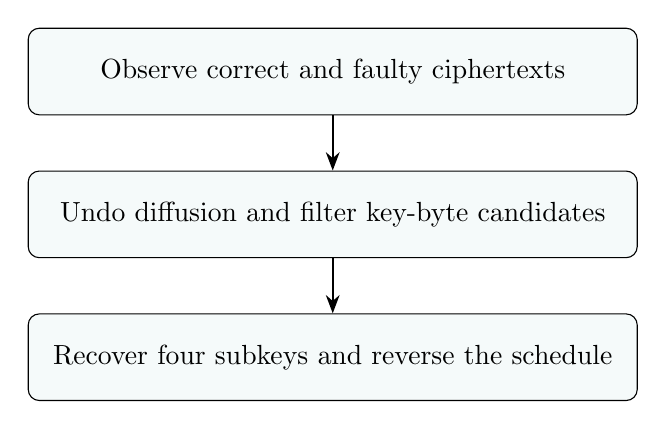
\begin{tikzpicture}[box/.style={draw,rounded corners,align=center,text width=75mm,minimum height=11mm,fill=teal!4},flow/.style={-{Stealth},thick}]
\node[box] (a) {Observe correct and faulty ciphertexts};
\node[box,below=7mm of a] (b) {Undo diffusion and filter key-byte candidates};
\node[box,below=7mm of b] (c) {Recover four subkeys and reverse the schedule};
\draw[flow] (a)--(b);\draw[flow] (b)--(c);
\end{tikzpicture}
\vfill
Guilherme Martins Specht\par
Industrial collaboration: STMicroelectronics\par
\vspace{8mm}
Independent guide --- \today\par
\end{titlepage}
\pagenumbering{roman}
\hypersetup{pageanchor=true}
\tableofcontents\clearpage
\pagenumbering{arabic}

\section{How to read the complete file}
This guide covers the imports, all eight top-level functions, the nested fault
callback, and the terminal entry point. It explains the purpose of each code
block, important operators and practical values. Repeated iterations are
summarized rather than printing 256 guesses or an entire matrix elimination.
The examples are checked by executing the current implementation when this PDF
is built. The source itself is not modified.

\note{\textbf{Scope.} The name ``Piret SM4'' identifies this project's controlled
known-byte DFA model. It is not an unchanged transfer of the historical AES
attack. Exact fault round, byte and XOR magnitude are simulation assumptions.
No physical STM32 key recovery is established by these Python examples.}

\subsection{The three roles that must remain separate}
\begin{center}\begin{tabular}{p{.22\linewidth}p{.68\linewidth}}\toprule
Role & What it knows and does\\\midrule
Simulated target & Knows plaintext and secret key; produces clean or faulted encryption.\\
Attacker / solver & Receives ciphertexts and permitted fault descriptors; filters candidates and recovers keys.\\
Teaching interface & Displays intermediate values to explain the simulation; these values must not become secret inputs to the solver.\\\bottomrule
\end{tabular}\end{center}

\subsection{Imports and representation}
\hx{argparse} handles command-line options. \hx{lru\_cache} stores the fixed inverse
matrix. \hx{struct} packs and unpacks four unsigned 32-bit words.
\hx{aes} supplies the shared block-length validator; this does not make the attack
an AES attack. \hx{sm4} supplies the public cipher, S-box, linear maps and constants.

The format \hx{">4I"} means four unsigned 32-bit integers in big-endian order.
Byte 0 is the most significant byte of a word. Bit index 0 in the binary matrix
is the least significant bit. The following operators have distinct roles:
\begin{center}\begin{tabular}{ll}\toprule
Python & Meaning here\\\midrule
\hx{a \^{} b} & XOR; addition/subtraction over GF(2)\\
\hx{a \& b} & Select bits; for sets, intersection\\
\hx{a | b} & Assemble bits in an integer\\
\hx{a << n}, \hx{a >> n} & Shift left/right by $n$ bits\\
\hx{a \% 4} & Wrap an integer index into 0, 1, 2, 3\\
\hx{items[::-1]} & Reverse a sequence\\\bottomrule
\end{tabular}\end{center}

\subsection{Running the example}
\begin{Verbatim}
python src/piret_sm4.py --step
python src/debug_piret_sm4.py
\end{Verbatim}
The first command presents the attack in the terminal. The second opens the
source-and-variables debugger with substituted numerical equations.

\section{\texorpdfstring{\texttt{sm4\_fault\_encrypt()}}{sm4_fault_encrypt}: simulate the target}
\subsection{Inputs and return values}
\hx{plaintext} and \hx{key} are 16-byte values. \hx{byte} is the affected S-box
byte, from 0 to 3; \hx{None} requests normal encryption. \hx{mask} is a nonzero
byte XOR error. \hx{fault\_round} is zero-based: 31 is the last of 32 rounds.
The return value is \hx{(ciphertext, trace)}. Only the ciphertext is returned
through the oracle to the recovery engine.

\subsection{Validate the requested fault}
When a byte is selected, the first condition checks the byte position and mask
range 1--255. The next condition requires a round in 0--31. Invalid descriptors
raise \hx{ValueError}; a missing fault byte disables injection.

\subsection{Prepare the teacher's trace}
\hx{sm4.key\_expansion(key)} creates the target's round keys. The loop builds one
trace dictionary per round, initially containing its index and round key.
The \hx{fields} dictionary translates event names into compact teaching labels:
S-box input $a$, S-box output $b$, linear output and new state word.
These keys and internal values belong to the target/teacher view, not the solver.

\subsection{Nested \texorpdfstring{\texttt{observer()}}{observer}: the exact fault instruction}
The cipher calls this callback at internal events. Its condition requires all
three properties: selected round, event \hx{"Sbox input"}, and a selected byte.
\begin{Verbatim}
value ^= mask << (24 - 8 * byte)
\end{Verbatim}
For byte 0 and mask 01, the shift is $24-8(0)=24$:
\[
\hex{01}\ll24=\texttt{01000000},\qquad
\texttt{96FF9D45}\xor\texttt{01000000}=\texttt{97FF9D45}.
\]
For byte 2 the shift is 8, so the same mask becomes \hx{00000100}.
The selected byte is corrupted before nonlinear substitution; XOR does not mean
replacing the entire byte with the mask.

If the event name is in \hx{fields}, the callback saves the value in that round's
trace. It returns the value, possibly changed. The real \hx{sm4.py} encryption
uses that returned value, which is what makes the intervention effective.
The final call passes this observer to \hx{sm4\_encrypt\_block}.

\note{A physical glitch changes operating conditions rather than executing this
XOR statement. A one-bit mask in Python is exact; a pulse on the board may cause
no error, multiple errors, an instruction fault or a reset.}

\section{\texorpdfstring{\texttt{inverse\_rows()}}{inverse_rows}: prepare inverse diffusion}
\subsection{Why this function exists}
The data linear map is
\[
L(x)=x\xor\rol_2(x)\xor\rol_{10}(x)\xor\rol_{18}(x)\xor\rol_{24}(x).
\]
It spreads the S-box output difference across a 32-bit word. The solver needs
the inverse map to restore that difference before guessing a key byte.
Linearity over GF(2) lets us write $y=Mx$ with a binary $32\times32$ matrix.
This function calculates $M^{-1}$, not a recovered secret.

\subsection{Cache the fixed matrix}
\begin{Verbatim}
@lru_cache(maxsize=1)
\end{Verbatim}
Because the matrix does not depend on the key or input, repeated calls reuse its
cached result. This lasts within the process until the cache is cleared or the
process ends; the comment ``first call, ever'' should be read with that limit.

\subsection{Step 1: discover each column}
\begin{Verbatim}
basis_word = 1 << bit_index
transformed_word = sm4.linear(basis_word)
columns.append(transformed_word)
\end{Verbatim}
The loop visits 32 unit vectors: \hx{00000001}, \hx{00000002}, \hx{00000004},
and so on. Applying $L$ to unit vector $i$ gives column $i$ of $M$.
For the first column:
\[
L(\texttt{00000001})=
\texttt{00000001}\xor\texttt{00000004}\xor\texttt{00000400}
\xor\texttt{00040000}\xor\texttt{01000000}=\texttt{01040405}.
\]
This column says which output bits depend on input bit 0.

\subsection{Step 2: collect rows and attach the identity}
\noindent\textbf{Goal:} take the already known matrix columns, reconstruct each
row, and attach an identity row. This step does not invert anything yet. The
result is the starting augmented matrix for the next step.

\begin{Verbatim}
rows = []
for row_index in range(32):
    matrix_row = 0
    for column_index in range(32):
        output_bit = (columns[column_index] >> row_index) & 1
        matrix_row |= output_bit << column_index
    identity_bit = 1 << (32 + row_index)
    augmented_row = matrix_row | identity_bit
    rows.append(augmented_row)
\end{Verbatim}
\noindent Indentation is essential: the identity is attached \emph{after} all
columns of one row have been read. The function appends one packed integer per
outer-loop iteration, not one integer per cell.

\subsubsection*{A drawing at the exact point where the bit is read}
Use a four-bit teaching matrix, with stored columns
$[\texttt{0101},\texttt{0011},\texttt{0010},\texttt{1000}]$ in binary.
The highlighted cell is row 1, column 1. Matrix rows run downward; matrix
columns run rightward. Printed binary numbers put bit 0 on the right.

\begin{center}
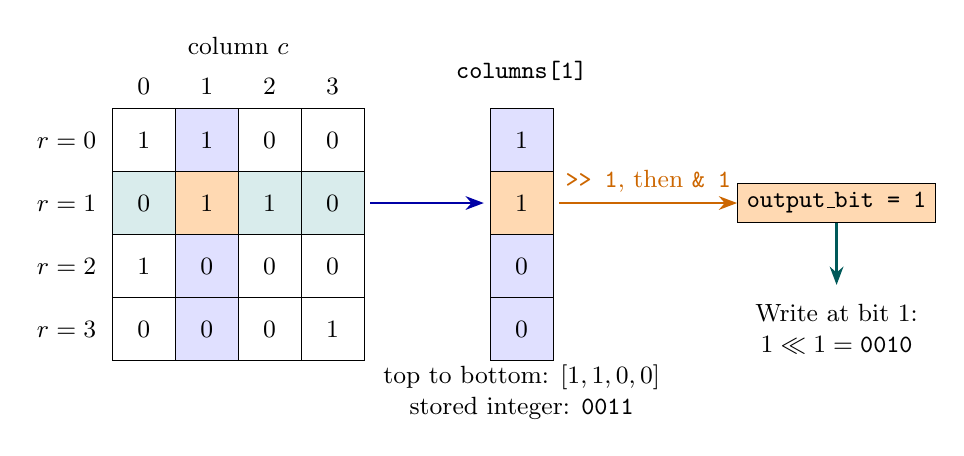
\begin{tikzpicture}[x=8mm,y=8mm,every node/.style={font=\small}]
\foreach \r/\a/\b/\c/\d in {0/1/1/0/0,1/0/1/1/0,2/1/0/0/0,3/0/0/0/1}{
\foreach \j/\v in {0/\a,1/\b,2/\c,3/\d}{
\def\shade{white}\ifnum\j=1\def\shade{blue!12}\fi
\ifnum\r=1\def\shade{teal!15}\fi
\ifnum\r=1\ifnum\j=1\def\shade{orange!30}\fi\fi
\node[draw,fill=\shade,minimum size=8mm] at (\j,-\r) {\v};}
\node[left] at (-.6,-\r) {$r=\r$};}
\foreach \j in {0,1,2,3}{\node at (\j,.85) {\j};}
\node at (1.5,1.5) {column $c$};
\foreach \r/\v in {0/1,1/1,2/0,3/0}{
\def\shade{blue!12}\ifnum\r=1\def\shade{orange!30}\fi
\node[draw,fill=\shade,minimum size=8mm] at (6,-\r) {\v};}
\node[align=center] at (6,1.1) {\hx{columns[1]}};
\draw[-{Stealth},thick,blue!65!black] (3.6,-1)--(5.4,-1);
\node[align=center] at (6,-4) {top to bottom: $[1,1,0,0]$\\stored integer: \hx{0011}};
\node[draw,fill=orange!30,align=center] (out) at (11,-1) {\hx{output\_bit = 1}};
\draw[-{Stealth},thick,orange!80!black] (6.6,-1)--node[above] {\hx{>> 1}, then \hx{\& 1}} (out.west);
\node[align=center] at (11,-3) {Write at bit 1:\\$1\ll1=\texttt{0010}$};
\draw[-{Stealth},thick,teal!70!black] (out.south)--(11,-2.3);
\end{tikzpicture}
\end{center}
The column is not moved. We read one coefficient from its packed integer and
write that coefficient into the packed row being constructed.

\subsubsection*{Every line: substituted values, result, and purpose}
For the small example only, use width 4 instead of 32 in the two ranges and in
the identity shift. The next worked iteration has $r=1$, $c=1$.
The preceding column $c=0$ contributed 0, so the accumulated row is still
\hx{0000}. Binary words below are padded to four or eight positions; loop
indices and shift counts are decimal.

\paragraph{1. \texttt{rows = []}.}
Create an empty list of augmented rows. It will eventually contain four
integers in this example, or 32 in SM4. The list is initialized once, before
either loop. It must retain earlier rows when a new row begins.

\paragraph{2. \texttt{for row\_index in range(4):}.}
The outer iterator produces $0,1,2,3$. We are showing its second iteration,
so \hx{row\_index = 1}. This selects the matrix row to reconstruct; it stays
fixed throughout the inner loop. Row 0 has already been appended.

\paragraph{3. \texttt{matrix\_row = 0}.}
At the beginning of row 1, set the accumulator to \hx{0000}. This removes the
bits used to construct the previous row; reusing that row would mix unrelated
coefficients. This line executes once per row, not once per column.

\paragraph{4. \texttt{for column\_index in range(4):}.}
Visit $c=0,1,2,3$ within fixed row $r=1$. At $c=1$, read the second stored
column: \hx{columns[1] = 0011}. The position in the list selects a column;
the row index selects a bit within that column.

\paragraph{5. \texttt{output\_bit = (columns[column\_index] >> row\_index) \& 1}.}
Substitute each operand:
\[
\begin{aligned}
\hx{output\_bit}&=(\texttt{0011}\gg1)\mathbin{\&}\texttt{0001}\\
&=\texttt{0001}\mathbin{\&}\texttt{0001}=1.
\end{aligned}
\]
Why shift? To bring the coefficient for row 1 into bit position 0.
Why AND with 1? To discard all other coefficients and obtain exactly 0 or 1.
For contrast, column 0 gives
$(\texttt{0101}\gg1)\mathbin{\&}\texttt{0001}
=\texttt{0010}\mathbin{\&}\texttt{0001}=0$.
The extra 1 in position 1 is irrelevant to this selected matrix entry.

\paragraph{6. \texttt{matrix\_row |= output\_bit << column\_index}.}
The augmented assignment is shorthand for
\hx{matrix\_row = matrix\_row | (output\_bit << column\_index)}.
For $c=1$ the complete update is
\[
\hx{matrix\_row}=\texttt{0000}\,|\,(1\ll1)
=\texttt{0000}\,|\,\texttt{0010}=\texttt{0010}.
\]
Why shift left? In the reconstructed row, column $c$ is stored at bit position
$c$. Why OR? Set that position while preserving all previously assembled bits.
In the next iteration $c=2$, another extracted 1 contributes \hx{0100}:
\[
\texttt{0010}\,|\,(1\ll2)
=\texttt{0010}\,|\,\texttt{0100}=\texttt{0110}.
\]
Column 3 contributes 0, so the completed row remains \hx{0110}.

\paragraph{7. \texttt{identity\_bit = 1 << (4 + row\_index)}.}
This line executes after the inner loop. Use $r=1$:
\[
\hx{identity\_bit}=1\ll(4+1)=1\ll5=\texttt{00100000}.
\]
Why add 4? The low four positions already hold the matrix row. The identity
must occupy the next four positions. Why add $r$? Row $r$ of the identity has
its 1 in column $r$. In SM4 this expression uses $32+r$, not $4+r$.

\paragraph{8. \texttt{augmented\_row = matrix\_row | identity\_bit}.}
Pad both operands to eight bits before combining them:
\[
\begin{array}{rcl}
\text{matrix row}&=&\texttt{0000\ 0110}\\
\text{identity row}&=&\texttt{0010\ 0000}\\\hline
\text{bitwise OR}&=&\texttt{0010\ 0110}.
\end{array}
\]
The result is decimal 38, hexadecimal \hx{26}. OR does not mean concatenating
decimal numbers: the two integers occupy non-overlapping bit positions.

\begin{center}
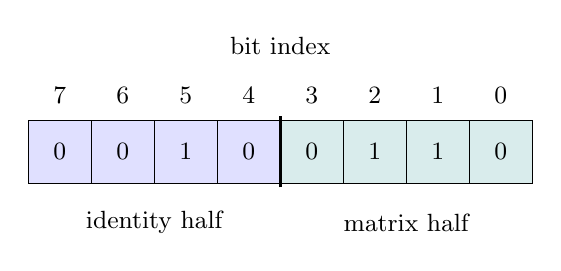
\begin{tikzpicture}[x=8mm,y=9mm,every node/.style={font=\small}]
\foreach \j/\b/\v in {0/7/0,1/6/0,2/5/1,3/4/0,4/3/0,5/2/1,6/1/1,7/0/0}{
\def\shade{blue!12}\ifnum\j>3\def\shade{teal!15}\fi
\node[draw,fill=\shade,minimum size=8mm] at (\j,0) {\v};
\node at (\j,.8) {\b};}
\node at (3.5,1.5) {bit index};
\draw[very thick] (3.5,-.5)--(3.5,.5);
\node at (1.5,-1) {identity half};\node at (5.5,-1) {matrix half};
\end{tikzpicture}
\end{center}
Mathematics writes $[M\mid I]$, but a printed integer lists its high half first,
so storage appears as $[I\mid M]$. The row operations will act on both halves.

\paragraph{9. \texttt{rows.append(augmented\_row)}.}
Row 0 previously produced \hx{00010011} (hex \hx{13}). Append row 1's
\hx{00100110} (hex \hx{26}):
\[
\hx{rows}=[\hx{13}]\quad\longrightarrow\quad[\hx{13},\hx{26}]
\qquad\text{(hexadecimal entries)}.
\]
Then the outer loop advances to row 2, resets the accumulator, and repeats.
This append is why completed rows are not lost when \hx{matrix\_row} is reset.

\subsubsection*{The complete four-bit run: every iteration, no guessed values}
In each table, $C$ is the stored column; ``shifted'' is $C\gg r$;
$b=(C\gg r)\mathbin{\&}1$; ``placed'' is $b\ll c$; and ``row before/after''
shows the OR accumulator. Padded digit strings are binary; the row and column
indices, shift counts and decimal shift results are ordinary decimal integers.
\paragraph{Outer iteration: row\_index = 0.}
Start with \hx{matrix\_row = 0000}.
\begin{center}\small\begin{tabular}{rllllll}\toprule
$c$ & $C$ & Shifted & $b$ & Placed & Row before & Row after\\\midrule
0 & 0101 & 0101 & 1 & 0001 & 0000 & 0001\\
1 & 0011 & 0011 & 1 & 0010 & 0001 & 0011\\
2 & 0010 & 0010 & 0 & 0000 & 0011 & 0011\\
3 & 1000 & 1000 & 0 & 0000 & 0011 & 0011\\
\bottomrule\end{tabular}\end{center}
\[\begin{aligned}
\hx{identity\_bit}&=1\ll(4+0)=16=\hx{00010000},\\
\hx{augmented\_row}&=\hx{00000011}\,|\,\hx{00010000}=\hx{00010011}.\end{aligned}\]
Append to \hx{rows}. List so far (hex): \hx{13}.
\paragraph{Outer iteration: row\_index = 1.}
Start with \hx{matrix\_row = 0000}.
\begin{center}\small\begin{tabular}{rllllll}\toprule
$c$ & $C$ & Shifted & $b$ & Placed & Row before & Row after\\\midrule
0 & 0101 & 0010 & 0 & 0000 & 0000 & 0000\\
1 & 0011 & 0001 & 1 & 0010 & 0000 & 0010\\
2 & 0010 & 0001 & 1 & 0100 & 0010 & 0110\\
3 & 1000 & 0100 & 0 & 0000 & 0110 & 0110\\
\bottomrule\end{tabular}\end{center}
\[\begin{aligned}
\hx{identity\_bit}&=1\ll(4+1)=32=\hx{00100000},\\
\hx{augmented\_row}&=\hx{00000110}\,|\,\hx{00100000}=\hx{00100110}.\end{aligned}\]
Append to \hx{rows}. List so far (hex): \hx{13, 26}.
\paragraph{Outer iteration: row\_index = 2.}
Start with \hx{matrix\_row = 0000}.
\begin{center}\small\begin{tabular}{rllllll}\toprule
$c$ & $C$ & Shifted & $b$ & Placed & Row before & Row after\\\midrule
0 & 0101 & 0001 & 1 & 0001 & 0000 & 0001\\
1 & 0011 & 0000 & 0 & 0000 & 0001 & 0001\\
2 & 0010 & 0000 & 0 & 0000 & 0001 & 0001\\
3 & 1000 & 0010 & 0 & 0000 & 0001 & 0001\\
\bottomrule\end{tabular}\end{center}
\[\begin{aligned}
\hx{identity\_bit}&=1\ll(4+2)=64=\hx{01000000},\\
\hx{augmented\_row}&=\hx{00000001}\,|\,\hx{01000000}=\hx{01000001}.\end{aligned}\]
Append to \hx{rows}. List so far (hex): \hx{13, 26, 41}.
\paragraph{Outer iteration: row\_index = 3.}
Start with \hx{matrix\_row = 0000}.
\begin{center}\small\begin{tabular}{rllllll}\toprule
$c$ & $C$ & Shifted & $b$ & Placed & Row before & Row after\\\midrule
0 & 0101 & 0000 & 0 & 0000 & 0000 & 0000\\
1 & 0011 & 0000 & 0 & 0000 & 0000 & 0000\\
2 & 0010 & 0000 & 0 & 0000 & 0000 & 0000\\
3 & 1000 & 0001 & 1 & 1000 & 0000 & 1000\\
\bottomrule\end{tabular}\end{center}
\[\begin{aligned}
\hx{identity\_bit}&=1\ll(4+3)=128=\hx{10000000},\\
\hx{augmented\_row}&=\hx{00001000}\,|\,\hx{10000000}=\hx{10001000}.\end{aligned}\]
Append to \hx{rows}. List so far (hex): \hx{13, 26, 41, 88}.


The loop terminates with four packed rows. Only now does Gaussian elimination
begin. No ciphertext, plaintext or secret key was needed to construct these
public matrix rows.

\subsubsection*{Back to real SM4: the exact same statements with width 32}
For \hx{row\_index = 1} and \hx{column\_index = 1}, the real column is
$L(2^1)=\hx{0208080A}$. The previous column gave a zero coefficient in this row,
so \hx{matrix\_row = 0}. Substitute the real values:
\[
\begin{aligned}
\hx{output\_bit}&=(\hx{0208080A}\gg1)\mathbin{\&}1\\
&=\hx{01040405}\mathbin{\&}1=1,\\
\hx{matrix\_row}&=\hx{00000000}\,|\,(1\ll1)=\hx{00000002}.
\end{aligned}
\]
The following table completes this real row across all 32 columns. Hexadecimal
is used for 32-bit words to avoid wrapping long binary strings; $b$ is a single
bit. Every cell extraction and accumulation is included for this one row.
\begingroup\small\begin{longtable}{rllrlll}\toprule
$c$ & $L(2^c)$ & Shifted by 1 & $b$ & Placed & Row before & Row after\\\midrule
\endhead
0 & 01040405 & 00820202 & 0 & 00000000 & 00000000 & 00000000\\
1 & 0208080A & 01040405 & 1 & 00000002 & 00000000 & 00000002\\
2 & 04101014 & 0208080A & 0 & 00000000 & 00000002 & 00000002\\
3 & 08202028 & 04101014 & 0 & 00000000 & 00000002 & 00000002\\
4 & 10404050 & 08202028 & 0 & 00000000 & 00000002 & 00000002\\
5 & 208080A0 & 10404050 & 0 & 00000000 & 00000002 & 00000002\\
6 & 41010140 & 208080A0 & 0 & 00000000 & 00000002 & 00000002\\
7 & 82020280 & 41010140 & 0 & 00000000 & 00000002 & 00000002\\
8 & 04040501 & 02020280 & 0 & 00000000 & 00000002 & 00000002\\
9 & 08080A02 & 04040501 & 1 & 00000200 & 00000002 & 00000202\\
10 & 10101404 & 08080A02 & 0 & 00000000 & 00000202 & 00000202\\
11 & 20202808 & 10101404 & 0 & 00000000 & 00000202 & 00000202\\
12 & 40405010 & 20202808 & 0 & 00000000 & 00000202 & 00000202\\
13 & 8080A020 & 40405010 & 0 & 00000000 & 00000202 & 00000202\\
14 & 01014041 & 0080A020 & 0 & 00000000 & 00000202 & 00000202\\
15 & 02028082 & 01014041 & 1 & 00008000 & 00000202 & 00008202\\
16 & 04050104 & 02028082 & 0 & 00000000 & 00008202 & 00008202\\
17 & 080A0208 & 04050104 & 0 & 00000000 & 00008202 & 00008202\\
18 & 10140410 & 080A0208 & 0 & 00000000 & 00008202 & 00008202\\
19 & 20280820 & 10140410 & 0 & 00000000 & 00008202 & 00008202\\
20 & 40501040 & 20280820 & 0 & 00000000 & 00008202 & 00008202\\
21 & 80A02080 & 40501040 & 0 & 00000000 & 00008202 & 00008202\\
22 & 01404101 & 00A02080 & 0 & 00000000 & 00008202 & 00008202\\
23 & 02808202 & 01404101 & 1 & 00800000 & 00008202 & 00808202\\
24 & 05010404 & 02808202 & 0 & 00000000 & 00808202 & 00808202\\
25 & 0A020808 & 05010404 & 0 & 00000000 & 00808202 & 00808202\\
26 & 14041010 & 0A020808 & 0 & 00000000 & 00808202 & 00808202\\
27 & 28082020 & 14041010 & 0 & 00000000 & 00808202 & 00808202\\
28 & 50104040 & 28082020 & 0 & 00000000 & 00808202 & 00808202\\
29 & A0208080 & 50104040 & 0 & 00000000 & 00808202 & 00808202\\
30 & 40410101 & 20208080 & 0 & 00000000 & 00808202 & 00808202\\
31 & 80820202 & 40410101 & 1 & 80000000 & 00808202 & 80808202\\
\bottomrule\end{longtable}\endgroup

After the last column, the result is \hx{80808202}. Its set positions are
1, 9, 15, 23 and 31. These are row coefficients, not the set positions in a
single column $L(2^c)$; rotations wrap around the word. Attach the identity:
\[
\begin{aligned}
\hx{identity\_bit}&=1\ll(32+1)=\hx{0000000200000000},\\
\hx{augmented\_row}&=\hx{0000000080808202}\,|\,\hx{0000000200000000}\\
&=\boxed{\hx{0000000280808202}}.
\end{aligned}
\]
The high 32 bits are \hx{00000002}, identity row 1; the low 32 bits are
\hx{80808202}, matrix row 1. This is a complete SM4 row, ready to append to
\hx{rows}. The other rows use their own row indices but exactly the same rule.


\subsection{Step 3: pivots and XOR elimination}
For each column, \hx{pivot = None} means that no suitable row has been found yet.
The search examines rows from the diagonal downward and stops at the first 1.
No pivot means a singular matrix; the current implementation raises
\hx{StopIteration}. Correct SM4 $L$ is invertible, so this is not a normal result.

The tuple assignment swaps the pivot into its diagonal position. The second
loop clears that column in every other row:
\begin{Verbatim}
rows[column], rows[pivot] = rows[pivot], rows[column]
rows[row] ^= rows[column]
\end{Verbatim}
Why XOR? Because $1\xor1=0$, exactly the cancellation required over GF(2).
The pivot is already 1, so division is unnecessary.

Here is the same method on a small $3\times3$ example, with conventional matrix
column order. This matrix is only an illustration, not a reduced SM4 cipher:
\[
\left[\begin{array}{ccc|ccc}
1&1&0&1&0&0\\0&1&1&0&1&0\\1&0&0&0&0&1
\end{array}\right]
\xrightarrow{R_2\gets R_2\xor R_0}
\left[\begin{array}{ccc|ccc}
1&1&0&1&0&0\\0&1&1&0&1&0\\0&1&0&1&0&1
\end{array}\right].
\]
Use row 1 to clear column 1 in rows 0 and 2:
\[
\left[\begin{array}{ccc|ccc}
1&0&1&1&1&0\\0&1&1&0&1&0\\0&0&1&1&1&1
\end{array}\right].
\]
Use row 2 to clear column 2 in rows 0 and 1:
\[
\left[\begin{array}{ccc|ccc}
1&0&0&0&0&1\\0&1&0&1&0&1\\0&0&1&1&1&1
\end{array}\right]=[I\mid M^{-1}].
\]
For instance, this inverse maps $(1,1,1)^T$ to $(1,0,1)^T$.
The real code performs the same operations for 32 columns.

\subsection{Step 4: extract the inverse rows}
\begin{Verbatim}
inverse_row = augmented_row >> 32
inverse_matrix_rows.append(inverse_row)
return tuple(inverse_matrix_rows)
\end{Verbatim}
The lower half is now the identity. Shifting by 32 discards it and keeps the
inverse row from the upper half. The tuple contains 32 integers, each encoding
one row of $M^{-1}$.

\section{\texorpdfstring{\texttt{inverse\_linear(value)}}{inverse_linear}: apply the inverse}
\subsection{The distinction from \texttt{inverse\_rows}}
\hx{inverse\_rows()} prepares the transformation. \hx{inverse\_linear(value)}
applies it to one observed 32-bit difference. The latter calls the former to
obtain its cached matrix, so callers do not need to prepare it manually.

\subsection{Follow one output bit}
\begin{Verbatim}
selected_bits = row & value
set_bit_count = bin(selected_bits).count("1")
parity = set_bit_count & 1
result |= parity << index
\end{Verbatim}
AND selects the participating input bits. Counting ones and keeping the low
count bit computes their parity: odd count gives 1, even count gives 0.
That is the GF(2) dot product of a matrix row and the input vector.
For \hx{value = 734E3D3D}, inverse row 0 gives
\[
\texttt{51154505}\mathbin{\&}\texttt{734E3D3D}=\texttt{51040505}.
\]
Eight selected bits are 1, so output bit 0 is $8\bmod2=0$.
Each of the 32 rows calculates one output bit. Shifting the parity positions
that bit, and OR assembles distinct positions without disturbing previous bits.
The complete result is
\[
\texttt{inverse\_linear(0x734E3D3D)}=\texttt{0x4F000000}.
\]
Applying forward $L$ returns \hx{734E3D3D}, which checks the inversion.

\clearpage
\section{Visual walkthrough: follow the loops through the matrix}
The drawings use a four-bit teaching matrix so every cell remains visible.
The real function uses the same indexing and operations with 32 bits. The small
matrix below is invertible, but it is not the SM4 linear transformation.

\definecolor{walkblue}{HTML}{DBEAFE}
\definecolor{walkteal}{HTML}{CCFBF1}
\definecolor{walkorange}{HTML}{FED7AA}
\newcommand{\walkmatrix}[2]{%
\begin{tikzpicture}[x=7mm,y=7mm,every node/.style={font=\small}]
\foreach \r/\a/\b/\c/\d in {0/1/1/0/0,1/0/1/1/0,2/1/0/0/0,3/0/0/0/1}{%
  \foreach \j/\v in {0/\a,1/\b,2/\c,3/\d}{%
    \def\shade{white}%
    \ifnum\j=#2\relax\def\shade{walkblue}\fi%
    \ifnum\r=#1\relax\def\shade{walkteal}\fi%
    \ifnum\r=#1\relax\ifnum\j=#2\relax\def\shade{walkorange}\fi\fi%
    \node[draw,fill=\shade,minimum width=7mm,minimum height=7mm] at (\j,-\r) {\v};%
  }%
  \node[left] at (-0.6,-\r) {$r=\r$};%
}%
\foreach \j in {0,1,2,3}{\node at (\j,0.9) {$\j$};}%
\node at (1.5,1.85) {\hx{column\_index}};
\draw[-{Stealth},thick,orange!80!black] (#2,1.5)--(#2,1.1);
\end{tikzpicture}}

\subsection{First understand the two directions}
\begin{center}
\walkmatrix{1}{2}
\end{center}
\begin{center}\begin{tabular}{ll}\toprule
Teal row & The outer loop fixes \hx{row\_index = 1}.\\
Blue column & The inner loop currently uses \hx{column\_index = 2}.\\
Orange cell & We read $M[1,2]=1$.\\\bottomrule
\end{tabular}\end{center}

\begin{Verbatim}
for row_index in range(4):        # move DOWN to the next row
    matrix_row = 0
    for column_index in range(4): # move RIGHT across this row
        output_bit = (columns[column_index] >> row_index) & 1
        matrix_row |= output_bit << column_index
\end{Verbatim}
\noindent The actual file uses \hx{range(32)}. While the inner loop runs,
\hx{row\_index} does not change. The visited cells are
\[
(0,0)\to(0,1)\to(0,2)\to(0,3),\quad
(1,0)\to(1,1)\to(1,2)\to(1,3),\quad\ldots
\]
The arrays already contain columns; these loops collect their bits into rows.
They do not move or modify the original matrix entries.

\subsection{Matrix order and printed binary order are different}
Matrix columns are drawn left-to-right as $c=0,1,2,3$. A printed binary integer
is written with its highest bit first: $b_3b_2b_1b_0$.
The highlighted matrix row is $[0,1,1,0]$. Its packed value is
$0\cdot2^0+1\cdot2^1+1\cdot2^2+0\cdot2^3=6$, printed as \hx{0110}.
For row 0, $[1,1,0,0]$ is printed as \hx{0011}, not \hx{1100}.
\note{A shift operates on the stored integer. It does not slide a matrix cell
visually to the right. The bit index tells us which coefficient to extract.}

\clearpage
\subsection{One column is an integer: why shift and AND?}
Column 0 of the teaching matrix contains these entries from top to bottom:
\begin{center}
\begin{tikzpicture}[x=12mm,y=9mm,every node/.style={font=\small}]
\foreach \r/\v in {0/1,1/0,2/1,3/0}{
\node[draw,fill=walkblue,minimum width=10mm,minimum height=8mm] at (0,-\r) {\v};
\node[left] at (-0.6,-\r) {row \r};
}
\node[align=left,anchor=west] at (1,-0.5) {row 0 $\to$ bit 0\quad(weight 1)\\row 1 $\to$ bit 1\quad(weight 2)\\row 2 $\to$ bit 2\quad(weight 4)\\row 3 $\to$ bit 3\quad(weight 8)};
\node[align=left,anchor=west] at (1,-2.5) {$1+0+4+0=5$\\\hx{columns[0] = 0b0101}};
\end{tikzpicture}
\end{center}
To read row 2 from this column, shift its bit into position 0, then keep only
that position. Every number below is a four-bit binary word:
\begin{center}
\begin{tikzpicture}[x=10mm,y=9mm,every node/.style={font=\small}]
\foreach \j/\bit in {0/3,1/2,2/1,3/0}{\node at (\j,0.9) {bit \bit};}
\foreach \j/\v in {0/0,1/1,2/0,3/1}{\node[draw,minimum size=8mm] at (\j,0) {\v};}
\node[right] at (4,0) {\hx{0101}: original column};
\foreach \j/\v in {0/0,1/0,2/0,3/1}{\node[draw,fill=walkteal,minimum size=8mm] at (\j,-1.5) {\v};}
\node[right] at (4,-1.5) {\hx{0001}: after \hx{>> 2}};
\draw[-{Stealth},orange!90!black,thick] (1,-0.45)--(3,-1.05);
\node[below,align=center] at (1.5,-2.3) {The selected bit reaches position 0.\\AND with \hx{0001} discards every other bit.};
\end{tikzpicture}
\end{center}
\[
(\texttt{0101}\gg2)\mathbin{\&}\texttt{0001}
=\texttt{0001}\mathbin{\&}\texttt{0001}=1.
\]
For row 1, instead:
\[
(\texttt{0101}\gg1)\mathbin{\&}\texttt{0001}
=\texttt{0010}\mathbin{\&}\texttt{0001}=0.
\]
The other surviving 1 in \hx{0010} does not matter: AND with 1 tests only the
least significant bit. This is why shifting alone is insufficient.

The four stored columns of this matrix are:
\begin{center}\begin{tabular}{ccccc}\toprule
Index & 0 & 1 & 2 & 3\\\midrule
Top-to-bottom entries & $[1,0,1,0]$ & $[1,1,0,0]$ & $[0,1,0,0]$ & $[0,0,0,1]$\\
Stored binary & \hx{0101} & \hx{0011} & \hx{0010} & \hx{1000}\\\bottomrule
\end{tabular}\end{center}

\clearpage
\subsection{Four iterations: build row 1 from left to right}
Keep \hx{row\_index = 1}. Start with \hx{matrix\_row = 0000}.
Each orange cell is the next bit read; all binary words below have four bits.

\noindent\begin{minipage}[t]{.48\linewidth}\centering
\textbf{Iteration 1: column 0}\par\medskip
\walkmatrix{1}{0}\par
Read $(\hx{0101}\gg1)\mathbin{\&}1=0$.\par
Position it: $0\ll0=\hx{0000}$.\par
Accumulate: $\hx{0000}\,|\,\hx{0000}=\hx{0000}$.
\end{minipage}\hfill
\begin{minipage}[t]{.48\linewidth}\centering
\textbf{Iteration 2: column 1}\par\medskip
\walkmatrix{1}{1}\par
Read $(\hx{0011}\gg1)\mathbin{\&}1=1$.\par
Position it: $1\ll1=\hx{0010}$.\par
Accumulate: $\hx{0000}\,|\,\hx{0010}=\hx{0010}$.
\end{minipage}

\bigskip\bigskip
\noindent\begin{minipage}[t]{.48\linewidth}\centering
\textbf{Iteration 3: column 2}\par\medskip
\walkmatrix{1}{2}\par
Read $(\hx{0010}\gg1)\mathbin{\&}1=1$.\par
Position it: $1\ll2=\hx{0100}$.\par
Accumulate: $\hx{0010}\,|\,\hx{0100}=\hx{0110}$.
\end{minipage}\hfill
\begin{minipage}[t]{.48\linewidth}\centering
\textbf{Iteration 4: column 3}\par\medskip
\walkmatrix{1}{3}\par
Read $(\hx{1000}\gg1)\mathbin{\&}1=0$.\par
Position it: $0\ll3=\hx{0000}$.\par
Accumulate: $\hx{0110}\,|\,\hx{0000}=\hx{0110}$.
\end{minipage}

\bigskip
The inner loop has reconstructed row 1: matrix entries $[0,1,1,0]$, stored as
integer 6, binary \hx{0110}. OR accumulates set bits; OR with zero preserves
the bits already written. Only after the inner loop finishes does the outer
loop move down to row 2 and reset \hx{matrix\_row = 0}.

\begin{center}
\begin{tikzpicture}[every node/.style={font=\small},node distance=4mm]
\node[draw,fill=walkblue,align=center] (a) {choose column\\\hx{columns[c]}};
\node[draw,fill=walkorange,right=of a,align=center] (b) {extract row bit\\\hx{>> r}, then \hx{\& 1}};
\node[draw,fill=walkteal,right=of b,align=center] (c) {place column bit\\\hx{<< c}, then OR};
\draw[-{Stealth}] (a)--(b);\draw[-{Stealth}] (b)--(c);
\end{tikzpicture}
\end{center}

\clearpage
\subsection{Where does the identity go in the packed row?}
With four bits per half, the code's \hx{32 + row\_index} becomes
\hx{4 + row\_index}. For row 1, the identity's 1 belongs at position 5:
\[
\hx{identity\_bit}=1\ll(4+1)=\texttt{00100000}.
\]
\begin{center}
\begin{tikzpicture}[x=9mm,y=10mm,every node/.style={font=\small}]
\foreach \j/\bit/\v in {0/7/0,1/6/0,2/5/1,3/4/0,4/3/0,5/2/1,6/1/1,7/0/0}{
\def\shade{walkblue}\ifnum\j>3\def\shade{walkteal}\fi
\node[draw,fill=\shade,minimum size=9mm] at (\j,0) {\v};
\node at (\j,.8) {\bit};
}
\draw[very thick] (3.5,-.5)--(3.5,.5);
\node at (1.5,-1) {high half: row of $I$};
\node at (5.5,-1) {low half: row of $M$};
\end{tikzpicture}
\end{center}
\[
\underbrace{\texttt{00000110}}_{\text{matrix row}}
\ \big|\ \underbrace{\texttt{00100000}}_{\text{identity bit}}
=\underbrace{\texttt{00100110}}_{\text{packed augmented row}}.
\]
Mathematics writes $[M\mid I]$, but the integer above is printed high-to-low
as $[I\mid M]$. This is a storage convention, not a different algorithm.
For 32-bit SM4 halves the same structure uses 64 bit positions.

\subsection{The elimination loop walks differently}
The \hx{column} loop now chooses a pivot column, rather than collecting a row.
\hx{candidate\_row} searches down that column from the diagonal.
After a pivot is found, \hx{row} scans all other rows to eliminate their 1s.
\begin{center}
\begin{tikzpicture}[x=11mm,y=9mm,every node/.style={font=\small}]
\foreach \r/\a/\b/\c/\d in {0/1/1/0/0,1/0/1/1/0,2/1/0/0/0,3/0/0/0/1}{
\foreach \j/\v in {0/\a,1/\b,2/\c,3/\d}{
\def\shade{white}\ifnum\j=0\def\shade{walkblue}\fi
\ifnum\r=0\def\shade{walkteal}\fi
\node[draw,fill=\shade,minimum width=11mm,minimum height=9mm] at (\j,-\r) {\v};}
\node[left] at (-.6,-\r) {$R_{\r}$};}
\node[right,align=left] at (4,0) {pivot row: keep it};
\node[right,align=left] at (4,-1) {column 0 is 0: skip};
\node[right,align=left] at (4,-2) {column 0 is 1: XOR pivot};
\node[right,align=left] at (4,-3) {column 0 is 0: skip};
\draw[-{Stealth},thick,orange!90!black] (-1.1,-.2)--(-1.1,-2);
\end{tikzpicture}
\end{center}
Here $R_2\gets R_2\xor R_0$. Its matrix entries change from
$[1,0,0,0]$ to $[0,1,0,0]$. Stored as integers, the XOR is
$\hx{0001}\xor\hx{0011}=\hx{0010}$. The identity half must change too:
\[
\texttt{01000001}\xor\texttt{00010011}=\texttt{01010010}.
\]
After all pivot columns, the low half is identity and the high half is inverse.
The final \hx{>> 4} (\hx{>> 32} in SM4) keeps the high half and discards the low.

\clearpage
\subsection{Finally, walk through the inverse matrix with the input vector}
For this teaching matrix, Gaussian elimination gives
\[
M^{-1}=\begin{bmatrix}
0&0&1&0\\1&0&1&0\\1&1&1&0\\0&0&0&1
\end{bmatrix}.
\]
Let $y=[1,1,1,0]^T$, stored as \hx{0111}. Each loop iteration selects one
inverse row and calculates a single output bit. This is a row--vector dot
product over GF(2), not another matrix inversion.
\begin{center}
\begin{tikzpicture}[x=7mm,y=8mm,every node/.style={font=\small}]
\foreach \r/\a/\b/\c/\d in {0/0/0/1/0,1/1/0/1/0,2/1/1/1/0,3/0/0/0/1}{
\foreach \j/\v in {0/\a,1/\b,2/\c,3/\d}{
\def\shade{white}\ifnum\r=1\def\shade{walkteal}\fi
\node[draw,fill=\shade,minimum width=7mm,minimum height=8mm] at (\j,-\r) {\v};}}
\foreach \r/\v in {0/1,1/1,2/1,3/0}{\node[draw,fill=walkblue,minimum width=7mm,minimum height=8mm] at (5,-\r) {\v};}
\node at (4,-1.5) {$\times$};
\node[right,align=left] at (6,-1.5) {Highlighted row 1:\\$(1\cdot1)\xor(0\cdot1)\xor(1\cdot1)\xor(0\cdot0)=0$};
\end{tikzpicture}
\end{center}

\begin{center}\begin{tabular}{cccccc}\toprule
Index & Packed row & Input & AND & Ones / parity & Running result\\\midrule
0 & \hx{0100} & \hx{0111} & \hx{0100} & 1 / 1 & \hx{0001}\\
1 & \hx{0101} & \hx{0111} & \hx{0101} & 2 / 0 & \hx{0001}\\
2 & \hx{0111} & \hx{0111} & \hx{0111} & 3 / 1 & \hx{0101}\\
3 & \hx{1000} & \hx{0111} & \hx{0000} & 0 / 0 & \hx{0101}\\\bottomrule
\end{tabular}\end{center}
The output is $x=[1,0,1,0]^T$, stored as \hx{0101}. Forward multiplication
$Mx$ restores $y=[1,1,1,0]^T$, so the inverse result is checked.

\begin{center}\begin{tabular}{p{.36\linewidth}p{.53\linewidth}}\toprule
Loop / operation & Picture to remember\\\midrule
\hx{bit\_index} & Feed one unit vector; obtain one column.\\
\hx{row\_index}, \hx{column\_index} & Fix a row; scan its cells left-to-right.\\
\hx{>> row\_index}, then \hx{\& 1} & Bring one column bit to position 0; isolate it.\\
\hx{<< column\_index}, then OR & Place that bit in the packed output row.\\
\hx{column}, \hx{candidate\_row} & Choose a pivot column; search downward.\\
\hx{rows[row] \^{}= rows[column]} & XOR the entire augmented row, both halves.\\
\hx{augmented\_row >> 32} & Keep the inverse half after elimination.\\
\hx{index, row} in \hx{inverse\_linear} & Select one inverse row; calculate one output bit.\\\bottomrule
\end{tabular}\end{center}
\note{In the real SM4 example, the same procedure gives
$L^{-1}(\hx{734E3D3D})=\hx{4F000000}$. The four-bit drawings illustrate storage
and traversal; they do not replace the real 32-bit map.}
\clearpage

\section{\texorpdfstring{\texttt{sm4\_byte\_candidates()}}{sm4_byte_candidates}: solve one observation}
\subsection{What the function receives}
Inputs are clean ciphertext, faulty ciphertext, selected byte and known mask.
Neither the target key nor its internal trace is an argument. After validating
lengths and ranges, \hx{struct.unpack(">4I", ...)} splits each output into words.
SM4 ciphertext order is $(X_{35},X_{34},X_{33},X_{32})$.

\subsection{Check the fault shape and undo L}
The check \hx{c[1:] != f[1:]} rejects changes in the other three words: the
isolated last-round model requires them unchanged. The function then computes
\[
\Delta X=c[0]\xor f[0],\qquad \Delta B=L^{-1}(\Delta X).
\]
For the first public-vector observation:
\[
\texttt{681EDF34}\xor\texttt{1B50E209}=\texttt{734E3D3D},
\qquad \Delta B=\texttt{4F000000}.
\]
These shape checks are model-consistency checks, not proof of a physical
single-bit error at the intended instruction.

\subsection{Select the byte and observable constant}
\begin{Verbatim}
shift = 24 - 8 * byte
d = (delta_b >> shift) & 255
known = ((c[1] ^ c[2] ^ c[3]) >> shift) & 255
\end{Verbatim}
For byte 0, \hx{shift = 24}, so $d=\hex{4F}$. The preceding condition rejects
zero differences and any bits outside the selected byte. In
\hx{delta\_b \& \~{}(255 << shift)}, complement creates a mask for all other
positions; AND detects unwanted differences there. Python's unbounded signed
complement is harmless for this test with a nonnegative 32-bit difference.

The known data-word XOR is
\[
\texttt{D206965E}\xor\texttt{86B3E94F}\xor\texttt{536E4246}
=\texttt{07DB3D57},
\]
so the first byte's observable constant is $q=\hex{07}$, stored as \hx{known}.
This XOR is the combination of the three newest input words, not the older
word canceled when forming the ciphertext difference.

\subsection{Try inputs, then convert them into key bytes}
\begin{Verbatim}
faulty_input = candidate_input ^ mask
output_difference = sm4.SBOX[candidate_input] ^ sm4.SBOX[faulty_input]
\end{Verbatim}
The loop visits 0--255 and keeps inputs satisfying
$S(a)\xor S(a\xor e)=d$. With $e=\hex{01}$ and $d=\hex{4F}$, the input guesses
are \hx{96} and \hx{97}:
\[
S(\hex{96})\xor S(\hex{97})=\hex{1A}\xor\hex{55}=\hex{4F}.
\]
Because $a=q\xor k$, the next loop computes \hx{key\_byte = candidate\_input \^{} known}:
\[
\hex{96}\xor\hex{07}=\hex{91},\qquad
\hex{97}\xor\hex{07}=\hex{90}.
\]
The return tuple contains key candidates, input candidates, and the full
\hx{delta\_b} word. One observation leaves ambiguity; this function does not
select the reference key from that ambiguity.

\section{\texorpdfstring{\texttt{reverse\_sm4()}}{reverse_sm4}: recover the master key}
\subsection{Why the input contains four subkeys}
The function requires four consecutive final subkeys in ascending order:
$rk_{28},rk_{29},rk_{30},rk_{31}$. They correspond to schedule words
$K_{32},K_{33},K_{34},K_{35}$.
\begin{Verbatim}
words = [None] * 32 + list(final_keys)
\end{Verbatim}
This creates 36 slots: 32 unknown words followed by four known seed words.
One 32-bit final subkey is insufficient for this direct recurrence inversion.

\subsection{Reverse one recurrence, then repeat}
\begin{Verbatim}
value = words[index+1] ^ words[index+2] ^ words[index+3] ^ sm4.CK[index]
words[index] = words[index+4] ^ sm4.linear_key(sm4.sbox(value))
\end{Verbatim}
The loop \hx{range(31, -1, -1)} visits 31 down to 0. At each step the four
words to the right are already known. It implements
\[
K_i=K_{i+4}\xor T'(K_{i+1}\xor K_{i+2}\xor K_{i+3}\xor CK_i).
\]
Here $T'=L'\circ\tau$, where $L'(z)=z\xor\rol_{13}(z)\xor\rol_{23}(z)$.
This is different from data diffusion $L$. The constants $CK_i$ are public:
byte $j$ is $7(4i+j)\bmod256$, with bytes concatenated big-endian.
For the first backward step ($i=31$), substitute the recovered words:
\begin{align*}
Q&=\hx{428D3654}\xor\hx{62293496}\xor\hx{01CF72E5}\xor\hx{646B7279}\\
&=\hx{4500025E},\\
\tau(Q)&=\hx{73D6E99D},\qquad T'(Q)=\hx{605CAC93},\\
K_{31}&=\hx{9124A012}\xor\hx{605CAC93}=\hx{F1780C81}.\end{align*}
The same rule repeats down to index 0; no further faulty encryptions are needed for this inversion.

The optional observer receives the newly calculated index and word for teaching.
It is not required to calculate the key.

\subsection{Remove FK and serialize}
\begin{Verbatim}
master_word = words[word_index] ^ sm4.FK[word_index]
return struct.pack(">4I", *master_words)
\end{Verbatim}
The initial words were whitened by fixed public constants, so XOR removes them.
The four results are serialized into the 16-byte master key. For word 0:
$\hex{A292FFA1}\xor\hex{A3B1BAC6}=\hex{01234567}$.
The star expands the four-word list into four arguments to \hx{struct.pack}.

\section{\texorpdfstring{\texttt{peel\_sm4()}}{peel_sm4}: expose an earlier round}
\subsection{Restore chronological order}
This function receives a ciphertext, a target round in 28--31 and a dictionary
containing only already recovered keys. It validates the block, unpacks its
four words and reverses their order:
\begin{Verbatim}
words = list(struct.unpack(">4I", ciphertext))[::-1]
\end{Verbatim}
Ciphertext order is reversed relative to the rolling cipher state. For the
public vector the chronological window is
\[
[\hex{536E4246},\hex{86B3E94F},\hex{D206965E},\hex{681EDF34}].
\]

\subsection{Undo only rounds with recovered keys}
For target round 31, \hx{range(31, 31, -1)} is empty: no round is peeled.
For target round 30, only round 31 is undone. If its key is missing,
the function raises \hx{ValueError} instead of guessing a key.
\begin{Verbatim}
previous = words[3] ^ sm4.linear(sm4.sbox(words[0] ^ words[1] ^ words[2] ^ recovered_keys[number]))
words = [previous, words[0], words[1], words[2]]
\end{Verbatim}
This solves the forward recurrence for the state word that was dropped.
Using recovered $rk_{31}=\hex{9124A012}$:
\[
A=\hex{536E4246}\xor\hex{86B3E94F}\xor\hex{D206965E}
\xor\hex{9124A012}=\hex{96FF9D45},
\]
\[
\tau(A)=\hex{1A488C73},\quad L(\tau(A))=\hex{138D5078},\quad
X_{31}=\hex{681EDF34}\xor\hex{138D5078}=\hex{7B938F4C}.
\]
The new chronological window is
\[
[\hex{7B938F4C},\hex{536E4246},\hex{86B3E94F},\hex{D206965E}].
\]
Finally the function reverses and packs it again, preserving the ciphertext-like
interface expected by the byte filter. The same peeling is applied separately
to correct and faulty outputs; teacher trace values are not used.

\section{\texorpdfstring{\texttt{recover\_sm4\_master\_key()}}{recover_sm4_master_key}: coordinate the attack}
\subsection{Inputs and validation}
\hx{correct} is the clean ciphertext. \hx{fault\_oracle(round, byte, mask)} asks
the target for a faulty ciphertext. \hx{masks} is converted to a tuple, then
checked for a nonempty sequence, distinct elements and values 1--255.
\hx{start\_byte} must be 0--3. Repeating the same mask on the same deterministic
input does not supply a new constraint, which motivates the duplicate check.

\hx{candidate\_filter=None} selects the known-mask filter described above.
A supplied filter can replace that equation, as in the Giraud-inspired adapter.
Its affected byte must match the requested byte. An optional \hx{observer}
receives copies of event dictionaries for presentation.

\subsection{Initialize state and choose byte order}
\hx{keys} stores uniquely recovered round keys; \hx{history} stores observation
records; \hx{counts} stores the latest surviving-candidate count for each byte;
\hx{used} counts faulty outputs.
The outer loop visits rounds 31, 30, 29 and 28. Each begins with a clean view
obtained by peeling only later rounds whose subkeys are in \hx{keys}.
\hx{bytearray(4)} allocates the four bytes of the current subkey.
\begin{Verbatim}
for offset in range(4):
    byte_order.append((start_byte + offset) % 4)
\end{Verbatim}
For \hx{start\_byte=2}, this gives
$(2+0)\bmod4=2$, $(2+1)\bmod4=3$, $(2+2)\bmod4=0$,
$(2+3)\bmod4=1$: order $[2,3,0,1]$.
This changes the visiting order, not byte positions in the assembled key.

\subsection{Ask for faults and intersect candidates}
For each byte, \hx{survivors=None} means no observation yet; it is not an empty
candidate set. \hx{enumerate(masks, 1)} provides observation numbers starting at 1
and their masks. The oracle returns a faulty ciphertext, it is peeled, and
the byte filter computes a fresh candidate set.
\begin{Verbatim}
if survivors is None:
    before = 256
    survivors = set(fresh)
else:
    before = len(survivors)
    survivors = survivors & fresh
\end{Verbatim}
With the first-byte example:
\[
\{\hex{90},\hex{91}\}\cap
\{\hex{70},\hex{72},\hex{93},\hex{91}\}=\{\hex{91}\}.
\]
The second set comes from mask 02 and difference 81. Intersection can remove
candidates but never introduce new ones. An empty intersection raises an error
because the observations are incompatible with the model.

\subsection{Record evidence; accept only uniqueness}
After each valid observation, \hx{used} increases and \hx{counts} is updated.
The event dictionary records round, byte, mask, counts, surviving values,
S-box inputs, inverse difference, ciphertexts, peeled views and the keys used
for peeling. It supports debugging and teaching; it is not an additional source
of secret key information.

\begin{Verbatim}
if len(survivors) == 1:
    subkey[byte] = next(iter(survivors))
    break
\end{Verbatim}
The set has exactly one element, so extracting that element is unambiguous.
\hx{break} stops requesting faults for this byte. It does not exit the round loop.
The \hx{else} attached to the observation \hx{for} executes only if its mask
budget is exhausted without that break. The function then returns
\hx{complete=False}, \hx{master\_key=None} and the blocked round; it never
pretends a guessed byte is recovered.

\subsection{Assemble subkeys, then reverse the schedule}
\begin{Verbatim}
keys[number] = int.from_bytes(subkey, "big")
\end{Verbatim}
For bytes \hx{91 24 A0 12}, this yields integer \hx{9124A012}.
Only after all four bytes are unique is the subkey available for peeling.
The final loop builds \hx{final\_keys} in ascending order 28--31, even though
the attack recovered them in descending order. It then calls
\hx{reverse\_sm4(final\_keys)} and returns the master key, four subkeys,
history, counts, query cost and \hx{complete=True}.
\begin{center}\begin{tabular}{ccc}\toprule
Recovered subkey & Value & Cumulative faulty outputs\\\midrule
$rk_{31}$ & \hx{9124A012} & 8\\
$rk_{30}$ & \hx{01CF72E5} & 16\\
$rk_{29}$ & \hx{62293496} & 24\\
$rk_{28}$ & \hx{428D3654} & 32\\
\bottomrule\end{tabular}\end{center}
This default-vector run uses 32 faulty outputs, plus the clean reference. It recovers $MK=\hx{0123456789ABCDEFFEDCBA9876543210}$. The observation count is an example result, not a universal physical requirement.


\section{\texorpdfstring{\texttt{main()}}{main}: connect the terminal interface}
\hx{ArgumentParser} reads command-line settings. The algorithm option is fixed
to SM4. \hx{--step} enables terminal lesson pauses; \hx{--color} controls ANSI
color; \hx{--faults} limits observations per byte; \hx{--row} chooses the first
byte to demonstrate. Its name is retained for interface compatibility, not
because SM4 uses an AES-style matrix.

\hx{--column} and \hx{--seed} are accepted for compatibility but are not forwarded
to \hx{run.sm4\_demo} by this entry point. They do not change this deterministic
SM4 scenario. The explicit fault-limit check rejects values outside 1--255.

The local \hx{import run} defers loading presentation until terminal execution
is requested. The call
\begin{Verbatim}
run.sm4_demo(run.LessonTerminal(args.color, args.step), args.faults, args.row)
\end{Verbatim}
connects settings to the existing shared lesson. Successful recovery returns
exit code 0; incomplete recovery returns 2.

\subsection{The final entry-point guard and logs}
\begin{Verbatim}
if __name__ == "__main__":
    from terminal_log import run_with_log
    raise SystemExit(run_with_log(main, "piret_sm4"))
\end{Verbatim}
This block runs when the file is executed directly. Importing the functions
does not launch a lesson. The wrapper captures terminal execution in
\hx{logs/piret\_sm4.txt} and colored HTML; files are overwritten per run.
\hx{SystemExit} passes the resulting status to the shell.

\clearpage
\section{Follow one real execution from the command to the recovered key}
This section is an execution route, not another independent description of the
functions. Read the numbered stages in order: the output of one call becomes
an input to the next. Numerical records are generated from the current solver.
The builder also runs the real terminal entry point without interactive pauses
and verifies that it succeeds. The command below adds pauses but follows the
same mathematical path:
\begin{Verbatim}
python src/piret_sm4.py --faults 8 --row 0 --step
\end{Verbatim}

\subsection{The route through the files}
\begin{center}
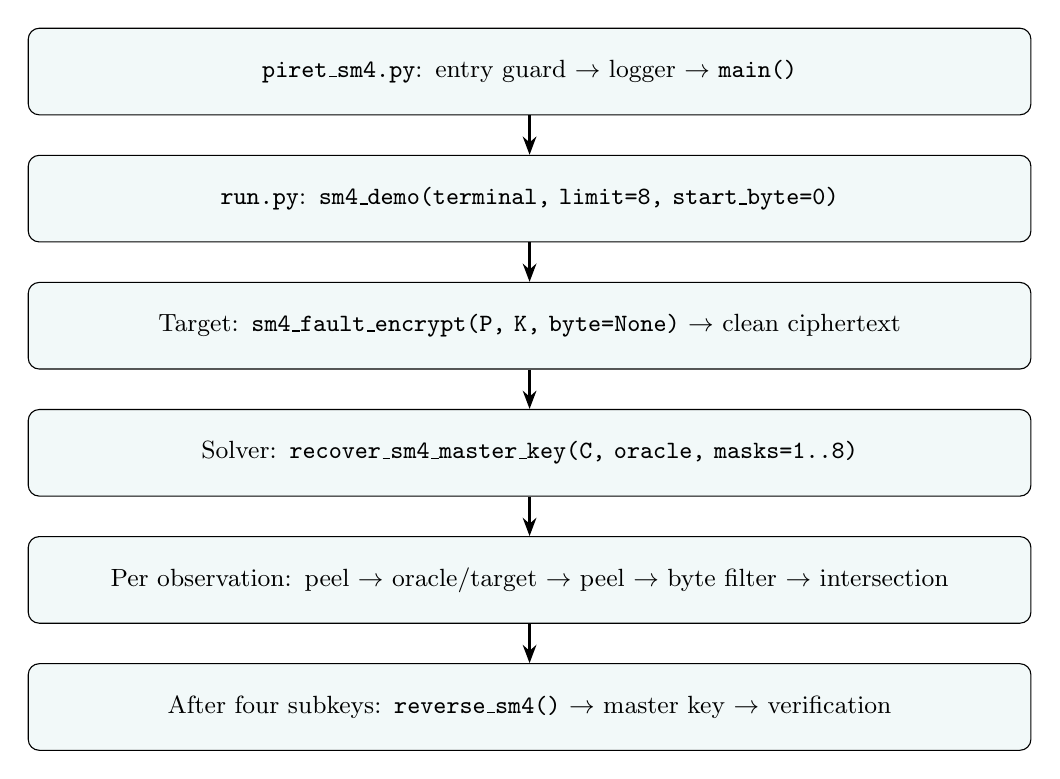
\begin{tikzpicture}[node distance=5mm,box/.style={draw,rounded corners,fill=teal!5,text width=125mm,align=center,minimum height=11mm,font=\small},flow/.style={-{Stealth},thick}]
\node[box] (a) {\hx{piret\_sm4.py}: entry guard $\to$ logger $\to$ \hx{main()}};
\node[box,below=of a] (b) {\hx{run.py}: \hx{sm4\_demo(terminal, limit=8, start\_byte=0)}};
\node[box,below=of b] (c) {Target: \hx{sm4\_fault\_encrypt(P, K, byte=None)} $\to$ clean ciphertext};
\node[box,below=of c] (d) {Solver: \hx{recover\_sm4\_master\_key(C, oracle, masks=1..8)}};
\node[box,below=of d] (e) {Per observation: peel $\to$ oracle/target $\to$ peel $\to$ byte filter $\to$ intersection};
\node[box,below=of e] (f) {After four subkeys: \hx{reverse\_sm4()} $\to$ master key $\to$ verification};
\draw[flow] (a)--(b);\draw[flow] (b)--(c);\draw[flow] (c)--(d);
\draw[flow] (d)--(e);\draw[flow] (e)--(f);
\end{tikzpicture}
\end{center}
The target knows the secret key. The solver receives ciphertexts and fault
descriptors. The terminal's teaching callbacks display additional internals;
their displays are not secret inputs to the candidate equations.

\subsection{Stage 1: argument parsing and the clean target call}
The entry guard calls \hx{run\_with\_log(main, "piret\_sm4")}. The parser obtains
\hx{faults=8}, \hx{row=0}, \hx{step=True}, with automatic color mode.
\hx{main()} constructs \hx{LessonTerminal} and invokes \hx{run.sm4\_demo}.
That function converts \hx{sm4.KEY} and \hx{sm4.PLAINTEXT} from hexadecimal
strings to bytes. For this public demonstration vector:
\[
P=K=\hx{0123456789ABCDEFFEDCBA9876543210}.
\]
The clean call uses \hx{byte=None}; the observer records events without
injecting any fault. The result is
\[
C=\hx{681EDF34D206965E86B3E94F536E4246}.
\]
The teacher can display the clean round-31 trace
$A=\hx{96FF9D45}$, $B=\hx{1A488C73}$, $L(B)=\hx{138D5078}$.
These values explain the target; the solver does not receive this trace.

\subsection{Stage 2: enter the solver and select the first byte}
The actual call passes \hx{range(1, 9)} as permitted masks and the two
callbacks \hx{oracle} and \hx{report}. Solver state starts as
\begin{Verbatim}
keys = {}
history = []
counts = {}
used = 0
\end{Verbatim}
The outer round loop selects \hx{number=31}. The call
\hx{peel\_sm4(C, 31, \{\})} undoes no rounds and returns $C$ unchanged.
The subkey buffer is \hx{00 00 00 00}; \hx{start\_byte=0} produces visiting
order $[0,1,2,3]$. The first selected byte is 0, \hx{survivors=None}, and
\hx{enumerate(masks, 1)} produces observation 1, mask 01.

\subsection{Stage 3: the oracle enters the target, then returns only ciphertext}
\begin{center}
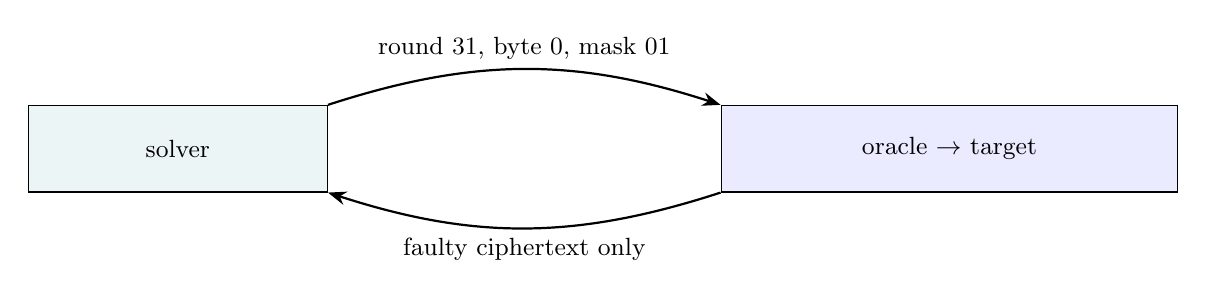
\begin{tikzpicture}[x=1mm,y=1mm,every node/.style={font=\small}]
\node[draw,fill=teal!8,minimum width=38mm,minimum height=11mm] (s) at (0,0) {solver};
\node[draw,fill=blue!8,minimum width=58mm,minimum height=11mm] (t) at (98,0) {oracle $\to$ target};
\draw[-{Stealth},thick] (s.north east) to[bend left=18] node[above] {round 31, byte 0, mask 01} (t.north west);
\draw[-{Stealth},thick] (t.south west) to[bend left=18] node[below] {faulty ciphertext only} (s.south east);
\end{tikzpicture}
\end{center}
\hx{oracle(31, 0, 1)} calls
\hx{sm4\_fault\_encrypt(P, K, byte=0, mask=1, fault\_round=31)}.
The callback intervenes only at the selected S-box input:
\[
\begin{aligned}
\text{shift}&=24-8(0)=24,\\
\text{shifted mask}&=\hx{01}\ll24=\hx{01000000},\\
A'&=\hx{96FF9D45}\xor\hx{01000000}=\hx{97FF9D45}.
\end{aligned}
\]
After the target completes normal SM4 processing, the oracle returns
\[
F_1=\hx{1B50E209D206965E86B3E94F536E4246}.
\]
The terminal may illustrate fault propagation using its teacher trace.
The solver gets $F_1$ alone. It calls \hx{peel\_sm4(F1,31,keys)}, which also
undoes no rounds.

\subsection{Stage 4: follow the first byte-filter call}
\hx{sm4\_byte\_candidates(C,F1,byte=0,mask=1)} unpacks four big-endian words
and checks that the last three words match. It computes
\[
\Delta X=\hx{681EDF34}\xor\hx{1B50E209}=\hx{734E3D3D}.
\]
Its call to \hx{inverse\_linear(0x734E3D3D)} obtains the fixed inverse rows.
On a fresh process, \hx{inverse\_rows()} builds and caches them; subsequent
observations reuse the matrix. The earlier illustrated matrix sections explain
that preparation. Applying its rows gives
\[
\Delta B=\hx{4F000000},\qquad
d=(\hx{4F000000}\gg24)\mathbin{\&}\hx{FF}=\hx{4F}.
\]
The other three words yield the public constant
\[
q_{\rm word}=\hx{D206965E}\xor\hx{86B3E94F}\xor\hx{536E4246}
=\hx{07DB3D57},\qquad q=\hx{07}.
\]
The 256-input loop retains only $a=\hx{96}$ and $a=\hx{97}$ because
$S(a)\xor S(a\xor\hx{01})=\hx{4F}$.
Converting input guesses to key guesses gives
$\hx{96}\xor\hx{07}=\hx{91}$ and
$\hx{97}\xor\hx{07}=\hx{90}$.
The function returns
\begin{Verbatim}
fresh  = {0x90, 0x91}
inputs = {0x96, 0x97}
delta  = 0x4F000000
\end{Verbatim}
Back in the solver, \hx{survivors=None} selects the first-observation branch:
\hx{before=256} and \hx{survivors=set(fresh)}.
\hx{used} becomes 1 and \hx{counts["31:0"]} becomes 2. An event is appended
and passed to \hx{report(event)} for display. Since two candidates remain,
the solver does not write a subkey byte yet.

\subsection{Stage 5: the second observation resolves the first byte}
The next observation requests \hx{oracle(31,0,2)}. It returns
\[
F_2=\hx{ED9DD932D206965E86B3E94F536E4246}.
\]
The same filter computes
\[
\begin{aligned}
\Delta X&=\hx{681EDF34}\xor\hx{ED9DD932}=\hx{85830606},\\
\Delta B&=L^{-1}(\hx{85830606})=\hx{81000000},\qquad d=\hx{81}.
\end{aligned}
\]
Its compatible S-box inputs are $\{\hx{75},\hx{77},\hx{94},\hx{96}\}$,
giving fresh key guesses $\{\hx{70},\hx{72},\hx{93},\hx{91}\}$.
The existing survivor set is now intersected:
\[
\{\hx{90},\hx{91}\}\cap\{\hx{70},\hx{72},\hx{93},\hx{91}\}
=\{\hx{91}\}.
\]
Now \hx{used=2}, \hx{counts["31:0"]=1} and \hx{subkey[0]=0x91}.
The buffer becomes \hx{91 00 00 00}; the other positions are not recovered yet.
The \hx{break} exits the mask loop, so mask 03 is not requested for this byte.

\subsection{Stages 6--9: follow all observations and assemble each subkey}
The next tables are generated from the real event history, in execution order.
They connect loop variables, inverse differences, candidate intersections,
byte-buffer updates and subkey milestones. All hexadecimal entries denote
values, not variable names. Query numbering excludes the clean reference.
\subsubsection*{Round 31: input views and the byte loop}
Before this round, recovered subkeys are:
\hx{none}.
The clean view returned by \texttt{peel\_sm4} is
\[C_{\rm view}=\hx{681EDF34D206965E86B3E94F536E4246}.\]
The first oracle response for this round and its peeled view are
\[\begin{aligned}F&=\hx{1B50E209D206965E86B3E94F536E4246},\\F_{\rm view}&=\hx{1B50E209D206965E86B3E94F536E4246}.\end{aligned}\]
The filter operates on these views. In the table, ``fresh'' is the key-byte set for this pair and ``remaining'' is the intersection with earlier observations for the same byte.
\begin{center}\small\begin{tabular}{rrrlll}\toprule
Query & Byte & Mask & $\Delta B$ & Fresh & Remaining\\\midrule
1 & 0 & 01 & 4F000000 & 90 91 & 90 91\\
2 & 0 & 02 & 81000000 & 70 72 91 93 & 91\\
3 & 1 & 01 & 00710000 & 24 25 & 24 25\\
4 & 1 & 02 & 00830000 & 24 26 & 24\\
5 & 2 & 01 & 00007900 & A0 A1 & A0 A1\\
6 & 2 & 02 & 00006F00 & A0 A2 & A0\\
7 & 3 & 01 & 00000080 & 12 13 & 12 13\\
8 & 3 & 02 & 000000C9 & 10 12 & 12\\
\bottomrule\end{tabular}\end{center}
Unique bytes are written into the subkey buffer in the following order. Zero-filled positions not yet written are placeholders, not recovered bytes.
\begin{center}\small\begin{tabular}{rrlr}\toprule
Byte written & Value & Buffer after write & Queries used\\\midrule
0 & 91 & 91000000 & 2\\
1 & 24 & 91240000 & 4\\
2 & A0 & 9124A000 & 6\\
3 & 12 & 9124A012 & 8\\
\bottomrule\end{tabular}\end{center}
Only now is \texttt{keys[31]} assigned: $rk_{31}=\hx{9124A012}$. This word may be used to peel the next attacked round.
\subsubsection*{Round 30: input views and the byte loop}
Before this round, recovered subkeys are:
\hx{rk31=9124A012}.
The clean view returned by \texttt{peel\_sm4} is
\[C_{\rm view}=\hx{D206965E86B3E94F536E42467B938F4C}.\]
For the clean ciphertext, the peeling calls perform the following actual calculations in order. The last column is the recovered older state word:
\begin{center}\small\begin{tabular}{rllll}\toprule
Undone round & S-box input & $\tau$ output & $L$ output & Older word\\\midrule
31 & 96FF9D45 & 1A488C73 & 138D5078 & 7B938F4C\\
\bottomrule\end{tabular}\end{center}
The first oracle response for this round and its peeled view are
\[\begin{aligned}F&=\hx{AE21A70A772712DA86B3E94F536E4246},\\F_{\rm view}&=\hx{772712DA86B3E94F536E42467B938F4C}.\end{aligned}\]
The filter operates on these views. In the table, ``fresh'' is the key-byte set for this pair and ``remaining'' is the intersection with earlier observations for the same byte.
\begin{center}\small\begin{tabular}{rrrlll}\toprule
Query & Byte & Mask & $\Delta B$ & Fresh & Remaining\\\midrule
9 & 0 & 01 & 21000000 & 00 01 & 00 01\\
10 & 0 & 02 & 3C000000 & 01 03 & 01\\
11 & 1 & 01 & 00550000 & CE CF & CE CF\\
12 & 1 & 02 & 006D0000 & CD CF & CF\\
13 & 2 & 01 & 00005100 & 72 73 & 72 73\\
14 & 2 & 02 & 0000AB00 & 70 72 & 72\\
15 & 3 & 01 & 000000EB & E4 E5 & E4 E5\\
16 & 3 & 02 & 000000FF & E5 E7 & E5\\
\bottomrule\end{tabular}\end{center}
Unique bytes are written into the subkey buffer in the following order. Zero-filled positions not yet written are placeholders, not recovered bytes.
\begin{center}\small\begin{tabular}{rrlr}\toprule
Byte written & Value & Buffer after write & Queries used\\\midrule
0 & 01 & 01000000 & 10\\
1 & CF & 01CF0000 & 12\\
2 & 72 & 01CF7200 & 14\\
3 & E5 & 01CF72E5 & 16\\
\bottomrule\end{tabular}\end{center}
Only now is \texttt{keys[30]} assigned: $rk_{30}=\hx{01CF72E5}$. This word may be used to peel the next attacked round.
\subsubsection*{Round 29: input views and the byte loop}
Before this round, recovered subkeys are:
\hx{rk31=9124A012, rk30=01CF72E5}.
The clean view returned by \texttt{peel\_sm4} is
\[C_{\rm view}=\hx{86B3E94F536E42467B938F4C893450AD}.\]
For the clean ciphertext, the peeling calls perform the following actual calculations in order. The last column is the recovered older state word:
\begin{center}\small\begin{tabular}{rllll}\toprule
Undone round & S-box input & $\tau$ output & $L$ output & Older word\\\midrule
31 & 96FF9D45 & 1A488C73 & 138D5078 & 7B938F4C\\
30 & AF8156A0 & 6FBFDA1D & 5B32C6F3 & 893450AD\\
\bottomrule\end{tabular}\end{center}
The first oracle response for this round and its peeled view are
\[\begin{aligned}F&=\hx{FD15CC075271D40B4F8E1DBB536E4246},\\F_{\rm view}&=\hx{4F8E1DBB536E42467B938F4C893450AD}.\end{aligned}\]
The filter operates on these views. In the table, ``fresh'' is the key-byte set for this pair and ``remaining'' is the intersection with earlier observations for the same byte.
\begin{center}\small\begin{tabular}{rrrlll}\toprule
Query & Byte & Mask & $\Delta B$ & Fresh & Remaining\\\midrule
17 & 0 & 01 & 3D000000 & 62 63 & 62 63\\
18 & 0 & 02 & 89000000 & 60 62 & 62\\
19 & 1 & 01 & 00E00000 & 28 29 & 28 29\\
20 & 1 & 02 & 001E0000 & 29 2B & 29\\
21 & 2 & 01 & 0000E900 & 34 35 & 34 35\\
22 & 2 & 02 & 00008200 & 34 36 & 34\\
23 & 3 & 01 & 00000057 & 96 97 & 96 97\\
24 & 3 & 02 & 0000001A & 94 96 & 96\\
\bottomrule\end{tabular}\end{center}
Unique bytes are written into the subkey buffer in the following order. Zero-filled positions not yet written are placeholders, not recovered bytes.
\begin{center}\small\begin{tabular}{rrlr}\toprule
Byte written & Value & Buffer after write & Queries used\\\midrule
0 & 62 & 62000000 & 18\\
1 & 29 & 62290000 & 20\\
2 & 34 & 62293400 & 22\\
3 & 96 & 62293496 & 24\\
\bottomrule\end{tabular}\end{center}
Only now is \texttt{keys[29]} assigned: $rk_{29}=\hx{62293496}$. This word may be used to peel the next attacked round.
\subsubsection*{Round 28: input views and the byte loop}
Before this round, recovered subkeys are:
\hx{rk31=9124A012, rk30=01CF72E5, rk29=62293496}.
The clean view returned by \texttt{peel\_sm4} is
\[C_{\rm view}=\hx{536E42467B938F4C893450AD6FE46B75}.\]
For the clean ciphertext, the peeling calls perform the following actual calculations in order. The last column is the recovered older state word:
\begin{center}\small\begin{tabular}{rllll}\toprule
Undone round & S-box input & $\tau$ output & $L$ output & Older word\\\midrule
31 & 96FF9D45 & 1A488C73 & 138D5078 & 7B938F4C\\
30 & AF8156A0 & 6FBFDA1D & 5B32C6F3 & 893450AD\\
29 & C3E0A931 & 928929B3 & E957823A & 6FE46B75\\
\bottomrule\end{tabular}\end{center}
The first oracle response for this round and its peeled view are
\[\begin{aligned}F&=\hx{84EB762070DAF490AA919B05476A5256},\\F_{\rm view}&=\hx{476A52567B938F4C893450AD6FE46B75}.\end{aligned}\]
The filter operates on these views. In the table, ``fresh'' is the key-byte set for this pair and ``remaining'' is the intersection with earlier observations for the same byte.
\begin{center}\small\begin{tabular}{rrrlll}\toprule
Query & Byte & Mask & $\Delta B$ & Fresh & Remaining\\\midrule
25 & 0 & 01 & 04000000 & 42 43 & 42 43\\
26 & 0 & 02 & 55000000 & 40 42 & 42\\
27 & 1 & 01 & 00820000 & 8C 8D & 8C 8D\\
28 & 1 & 02 & 00450000 & 8D 8F & 8D\\
29 & 2 & 01 & 00005800 & 36 37 & 36 37\\
30 & 2 & 02 & 00006000 & 34 36 & 36\\
31 & 3 & 01 & 00000096 & 54 55 & 54 55\\
32 & 3 & 02 & 00000022 & 54 56 & 54\\
\bottomrule\end{tabular}\end{center}
Unique bytes are written into the subkey buffer in the following order. Zero-filled positions not yet written are placeholders, not recovered bytes.
\begin{center}\small\begin{tabular}{rrlr}\toprule
Byte written & Value & Buffer after write & Queries used\\\midrule
0 & 42 & 42000000 & 26\\
1 & 8D & 428D0000 & 28\\
2 & 36 & 428D3600 & 30\\
3 & 54 & 428D3654 & 32\\
\bottomrule\end{tabular}\end{center}
Only now is \texttt{keys[28]} assigned: $rk_{28}=\hx{428D3654}$. The four required subkeys are now known; leave the round loop and reverse the key schedule.


\subsection{Stage 10: four recovered words enter reverse expansion}
The attack's recovery order was 31, 30, 29, 28. The final list is deliberately
assembled in the ascending order expected by \hx{reverse\_sm4}:
\begin{Verbatim}
final_keys = [0x428D3654, 0x62293496, 0x01CF72E5, 0x9124A012]
\end{Verbatim}
These are $K_{32},K_{33},K_{34},K_{35}$. The first backward calculation is
\[
\begin{aligned}
Q&=\hx{428D3654}\xor\hx{62293496}\xor\hx{01CF72E5}\xor\hx{646B7279}
=\hx{4500025E},\\
\tau(Q)&=\hx{73D6E99D},\qquad T'(Q)=\hx{605CAC93},\\
K_{31}&=\hx{9124A012}\xor\hx{605CAC93}=\hx{F1780C81}.
\end{aligned}
\]
Each following index reuses words already calculated to its right. No new
oracle requests occur in this phase. At the end, remove the four FK words:
\begin{center}\begin{tabular}{rlll}\toprule
$i$ & $K_i$ & $FK_i$ & $MK_i=K_i\oplus FK_i$\\\midrule
0 & A292FFA1 & A3B1BAC6 & 01234567\\
1 & DF01FEBF & 56AA3350 & 89ABCDEF\\
2 & 99A12B0F & 677D9197 & FEDCBA98\\
3 & C42410CC & B27022DC & 76543210\\
\bottomrule\end{tabular}\end{center}
Concatenation returns the 16 bytes \hx{0123456789ABCDEFFEDCBA9876543210}.


\subsection{Stage 11: return values, verification and process exit}
The solver returns \hx{complete=True}, the recovered master key, four subkeys,
32 events, candidate counts and \hx{used=32}. The terminal's schedule display
must agree with that key. The verified round trip is
\[
\begin{aligned}
\operatorname{Encrypt}(P,MK)&=\hx{681EDF34D206965E86B3E94F536E4246}=C,\\
\operatorname{Decrypt}(C,MK)&=\hx{0123456789ABCDEFFEDCBA9876543210}=P.
\end{aligned}
\]
The simulation also compares the recovered key with the target's reference
key, only for validation. \hx{sm4\_demo} returns \hx{True}; \hx{main} returns
0; the logging wrapper finishes and \hx{SystemExit} passes status 0 to the shell.
\note{The 32 faulty ciphertexts are this software example's recovery cost.
Teacher callbacks may recompute values for display; those calculations are not
additional independent observations. Physical glitch calibration and failed
acquisitions are not counted or demonstrated here.}
\clearpage

\section{One complete practical story}
The target encrypts a public plaintext with its hidden key. The solver gets a
clean ciphertext. It requests two useful fault observations for the first byte,
undoes $L$, intersects candidates and obtains 91. It repeats for the remaining
three bytes to obtain $rk_{31}$. Only then can it peel round 31 and attack round
30. The process continues through round 28. Four consecutive recovered subkeys
seed reverse expansion, whose initial FK whitening is undone to obtain the
master key. Re-encryption and decryption verify the result.

The source's known-mask solver and the physical injection mechanism are separate
questions. A valid laboratory evaluation must establish whether real faults
match the assumed round, location and magnitude; the exact XOR in the Python
callback is a controlled teaching model.

\subsection{Build this document}
\begin{Verbatim}
python build_piret_sm4_guide.py
\end{Verbatim}
\subsection{Source and verification record}
This edition covers all eight top-level functions and the nested observer in \texttt{src/piret\_sm4.py}. Source SHA-256: \url{424717e680ab76021831a9a6eaa490161342f43b21d4c8d086297ee97c051032}.
Its generated examples were checked using an actual complete recovery, matrix/parity checks, candidate intersections, peeling, re-encryption and decryption.

\end{document}
